\begin{frame}{Оценочная функция}
Для вычисления оценочной функции цепочки необходимы: \\
$ep_{chain} \left(n\right) \in 2^{\mathtt{Pieces}}$ --- множество фигур, участвующих в размене на $n$-ом поле траектории. \\
$value\left(p\right) \in \mathbb{Z}$ --- стоимость фигуры, белые фигуры имеют положительную оценку, черные -- отрицательную.\\ 
$len_{chain}\left(traj\right) \in \mathbb{N}^+$ --- длина траектории. \\
Определим оценочную функцию $\varphi \colon \mathtt{Chains} \to \mathbb{N}$:
$$
 \varphi \left( ch \right) = \sum_{k \in \left[0, l\right]} \sum_{ p \in ep\left(k\right)} value\left(p\right) + \sum_{sch \in sa\left(k, traj\right)} \varphi\left(sch\right)
$$
Согласно полученной оценке, построим граф, узлами которого являются оцененные цепочки, имеющие одинаковую изначальную структуру - подцепочку-0.
\end{frame}

\begin{frame}{Граф цепочек}
 Если две цепочки $\left(\Gamma_{0, 0}, \alpha_0\right)$ и $\left(\Gamma_{0, 1}, \alpha_1\right)$ таковы, что $\alpha_0 > \alpha_1$, то проводится ребро черного цвета. Это означает, что черные могут улучшить оценку в свою пользу. 
%\begin{tabular}{ll}
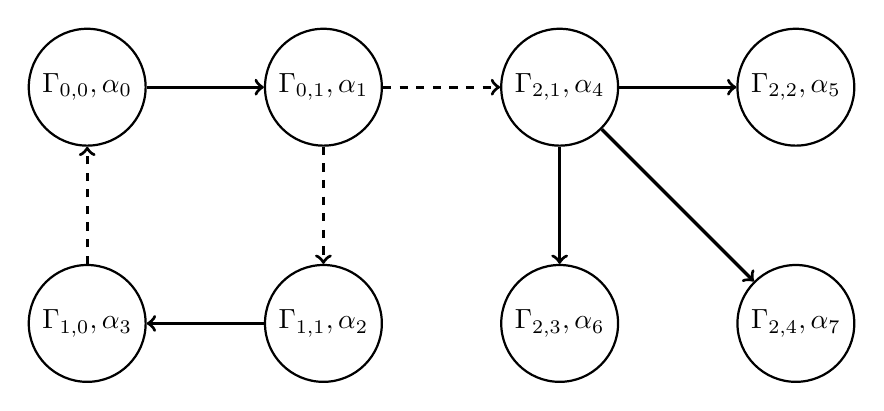
\begin{tikzpicture}
\begin{scope}[every node/.style={circle,thick,draw}]
    \node (00) at (0,0) {$\Gamma_{0, 0}, \alpha_0$};
    \node (01) at (3,0) {$\Gamma_{0, 1}, \alpha_1$};
    \node (21) at (6,0) {$\Gamma_{2, 1}, \alpha_4$};
    \node (11) at (3,-3) {$\Gamma_{1, 1}, \alpha_2$};
    \node (10) at (0,-3) {$\Gamma_{1, 0}, \alpha_3$};
    \node (22) at (9,0) {$\Gamma_{2, 2}, \alpha_5$};
    \node (23) at (6,-3) {$\Gamma_{2, 3}, \alpha_6$};
    \node (24) at (9,-3) {$\Gamma_{2, 4}, \alpha_7$};
\end{scope}
\begin{scope}[%>={Stealth[black]},
              every node/.style={fill=white,circle},
              every edge/.style={draw=black,very thick}]
    % подцепочка 0
    \path [->] (00) edge (01);
    \path [->] (11) edge (10);
    \path [->] (21) edge (22);
    \path [->] (21) edge (23);
    \path [->] (21) edge (24);
    \path [->] (01) edge[dashed] (21);
    \path [->] (01) edge[dashed] (11);
    \path [->] (10) edge[dashed] (00);
\end{scope}
\end{tikzpicture}
%&\end{tabular}
\end{frame}

\begin{frame}{Оптимальная цепочка}
Выбор цепочки с нашей стороны определяется максимальным значением оценочной функции, в то время как противник, наоборот, стремится реализовать цепочку, которая её минимизирует. \\
То есть, противник выбирает цепочку той же структуры нашего цвета, заменяя в ней подцепочки своего цвета, чтобы максимально уменьшить оценку. \\
В случае цикла, \textbf{оптимальным} считается тот узел, в котором при наилучшем выборе противника, мы имеем возможность улучшить оценку. \\
При линейной структуре \textbf{оптимальна} листовая вершина с максимальной оценкой.
\end{frame}

\begin{frame}{Трудности нахождения оптимальной цепочки} %граф, содержащий всё.
Основная трудность заключается в построении графа цепочек, так как при построении необходимо включать в него всевозможные цепочки. \\
Вместо полного перебора вариантов, хотелось бы иметь структуру, достраивающую подцепи динамически, если возникает такая необходимость.\\
Так же оценка фигур не является фиксированным числом, а зависит от цепочек, в которых она участвует. \\
Одна и та же фигура в одной цепочке может выполнять несколько функций, то есть, участвовать в нескольких подцепочках. В зависимости от временных рамок, её поведение так же может различаться. 
%Непонятно об оценке фигур и связях между фигурами в цепочках (в двух подцепях по-разному, можно ли ходить вдоль траектории, или нельзя).
\end{frame}

\endinput
\begin{frame}{Результаты}
{{$$\begin{cases}
\alpha_0 < \alpha_1 \\
\alpha_1 > \alpha_2 \\
\alpha_2 < \alpha_3 \\
\alpha_3 > \alpha_0
\end{cases}
$$}}
На данный момент программная реализация: \\
\begin{itemize}
\item находит пути на пустой доске (подцепи-0); \\
\item маркирует поля траектории по признаку проходимости; \\
\item находит кандидатные подцепи. \\
\end{itemize}
\end{frame}
